\documentclass[fleqn]{scrartcl}
\usepackage{graphicx}
\usepackage[T1]{fontenc}
\usepackage[utf8]{inputenc}
\usepackage{lmodern}
\usepackage{xspace}
\usepackage{tikz}
\usepackage[range-phrase = --,retain-unity-mantissa = false,exponent-product = \cdot]{siunitx}
\usepackage{url}
\newcommand{\email}[1]{\url{#1}}
\usetikzlibrary{calc}
\usetikzlibrary{datavisualization}
\usetikzlibrary{decorations}
\usepgflibrary{decorations.pathmorphing}

\usepackage[pdftitle={Pendent drop measurement with ImageJ},
    pdfauthor={Adrian Daerr and Adrien Mogne},
    pdfsubject={Pendent drop Plugin for ImageJ, Université Paris Diderot},
    pdfkeywords={pendent drop, surface tension, ImageJ},
    linkcolor=blue,pdfborder={0 0 0},citecolor=black,
    filecolor=blue,urlcolor=blue]{hyperref}

% Alter some LaTeX defaults for better treatment of figures:
  % source: http://mintaka.sdsu.edu/GF/bibliog/latex/floats.html
  % See p.105 of "TeX Unbound" for suggested values.
  % See pp. 199-200 of Lamport's "LaTeX" book for details.
  %   General parameters, for ALL pages:
  \renewcommand{\topfraction}{0.9}	% max fraction of floats at top
  \renewcommand{\bottomfraction}{0.8}	% max fraction of floats at bottom
  %   Parameters for TEXT pages (not float pages):
  \setcounter{topnumber}{2}
  \setcounter{bottomnumber}{2}
  \setcounter{totalnumber}{4}     % 2 may work better
  \setcounter{dbltopnumber}{2}    % for 2-column pages
  \renewcommand{\dbltopfraction}{0.9}	% fit big float above 2-col. text
  \renewcommand{\textfraction}{0.07}	% allow minimal text w. figs
  %   Parameters for FLOAT pages (not text pages):
  \renewcommand{\floatpagefraction}{0.7}	% require fuller float pages
  % N.B.: floatpagefraction MUST be less than topfraction !!
  \renewcommand{\dblfloatpagefraction}{0.7}	% require fuller float pages

\setcapindent{1em}

\newcommand{\gouttependante}{\texttt{Pendent\_Drop}\xspace}
\newcommand{\ud}{\mathrm{d}}% d droit
\newcommand{\grid}[2]{%
  \draw[step=0.1cm,gray,ultra thin] (-#1,-#2) grid (#1,#2);%
  \draw[step=0.5cm,gray,thin] (-#1,-#2) grid (#1,#2);%
  \draw[thick] (-#1,0) -- (#1,0);
  \draw[thick] (0,-#2) -- (0,#2);
}
\newcommand{\subfig}[1]{\textbf{\textsf{#1}}}

\begin{document}

\subject{\gouttependante}

\title{Measuring liquid surface tension through the
       pendent drop method: description of a measurement bench and an
       ImageJ Plugin}

\author{Adrian Daerr%
        \footnote{\email{adrian.daerr@univ-paris-diderot.fr}} \and
        Adrien Mogne}

\date{\scriptsize Matière et Systèmes Complexes UMR 7057,
      Université Paris Diderot, 75205 Paris cedex 13, France}

\maketitle

\begin{abstract}
  The pendent drop method for surface tension measurement consists in
  analysing the shape of an axisymmetric drop hanging from a capillary
  tube (Fig.~\ref{fig:pendentdropphoto}). This article describes the
  principle and some practical considerations in implementing this
  method, both experimentally and numerically. Our numerical tool to
  match a theoretical profile to the contour of a pendent drop, either
  interactively or automatically, is available as an open-source
  \gouttependante Plugin for
  \href{http://imagej.nih.gov/ij/}{ImageJ}~\cite{ImageJ}. This Plugin
  provides an estimate of the surface tension and other drop
  characteristics such as volume and surface area from the best
  matching parameters. We also present static and dynamic surface
  tension measurements on various liquids and a biosurfactant solution
  showing that this Plugin calculates values in accordance with known
  surface tensions and with those obtained via a commercial apparatus.
\end{abstract}


\begin{figure}
\center
  \begin{tikzpicture}[label/.style={inner sep=0.5em,color=white,anchor=south west}, photo/.style={inner sep=1pt, inner ysep=1pt}]
    \node[photo] (captube) 
      {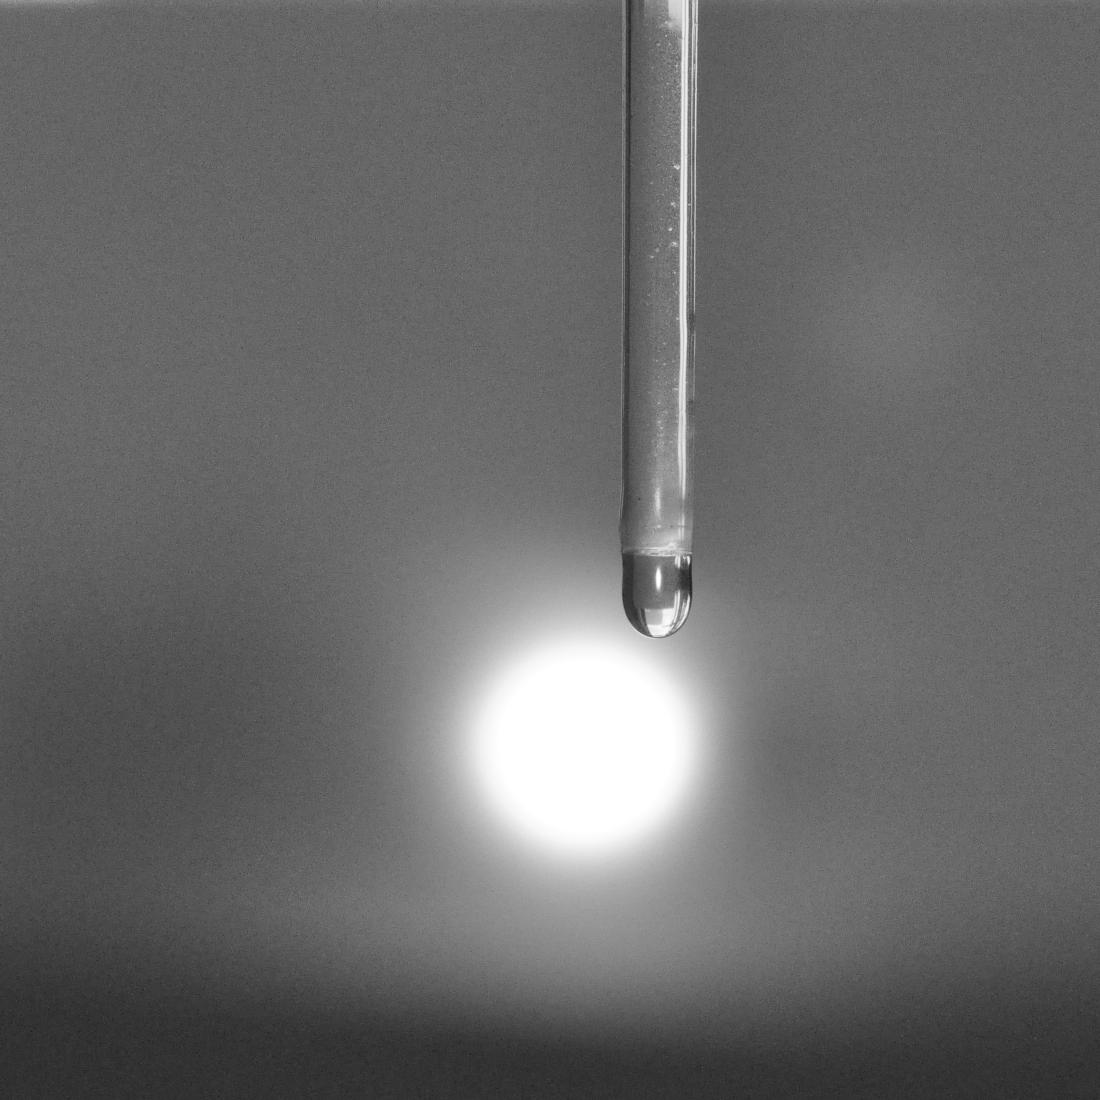
\includegraphics[height=170pt]{photogoutte1}} ;
    \node[label] (a) at (captube.south west) {\subfig{a}} ;
    \node[photo, anchor=north west] (waterraw) at (captube.north east)
      {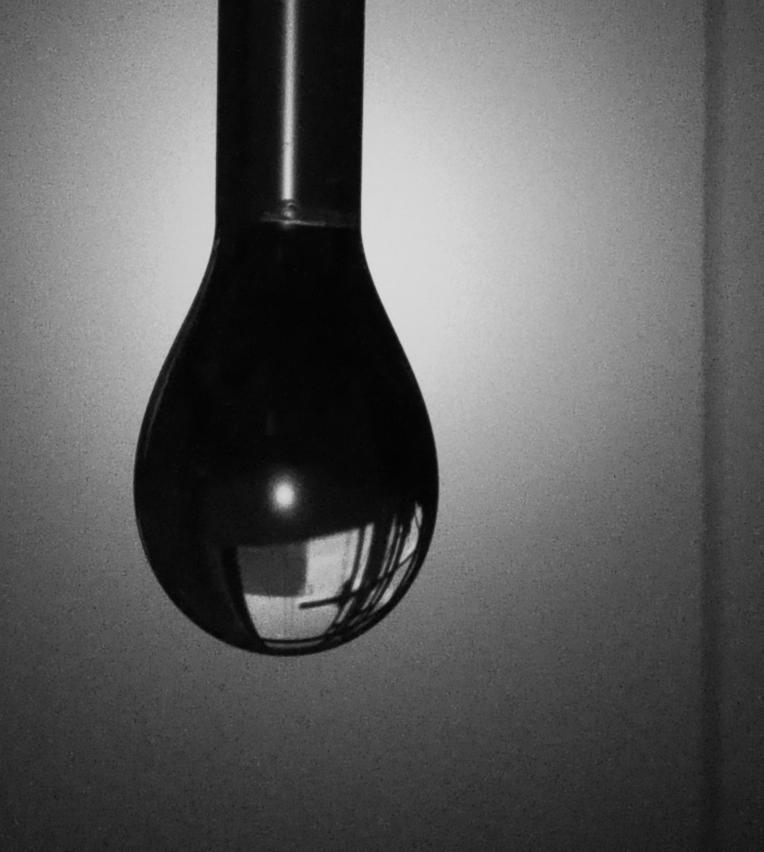
\includegraphics[height=84pt]{photogoutte3}} ;
    \node[label] (b) at (waterraw.south west) {\subfig{b}} ;
    \node[photo, anchor=north west] (siliconoilraw) at (waterraw.north east)
      {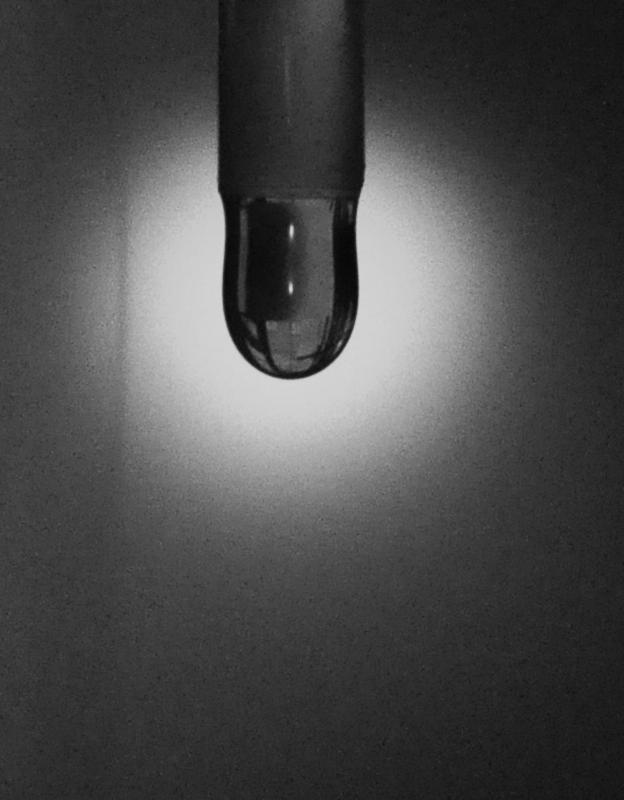
\includegraphics[height=84pt]{photogoutte2}} ;
    \node[label] (c) at (siliconoilraw.south west) {\subfig{c}} ;
    \node[photo, anchor=north west] (wateroptim) at (waterraw.south west)
      {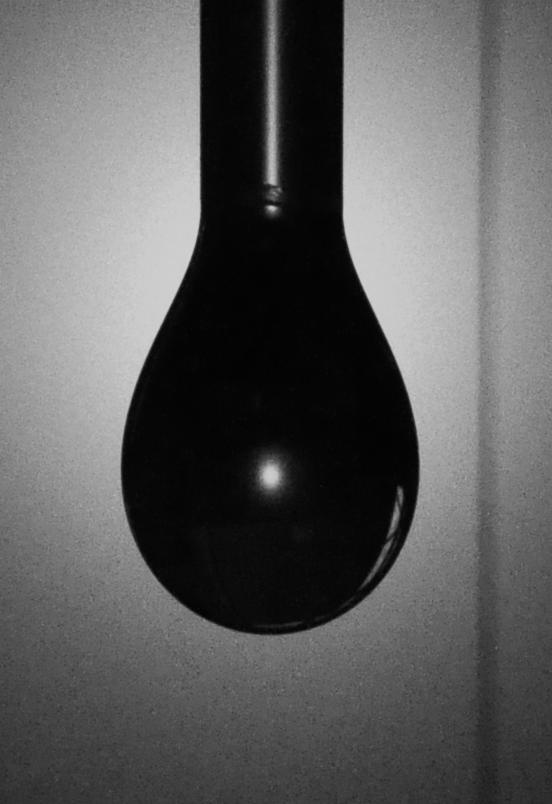
\includegraphics[height=84pt]{photogoutte5}} ;
    \node[label] (d) at (wateroptim.south west) {\subfig{d}} ;
    \node[photo, anchor=south east] (siliconoiloptim)
      at (siliconoilraw.east |- wateroptim.south)
      {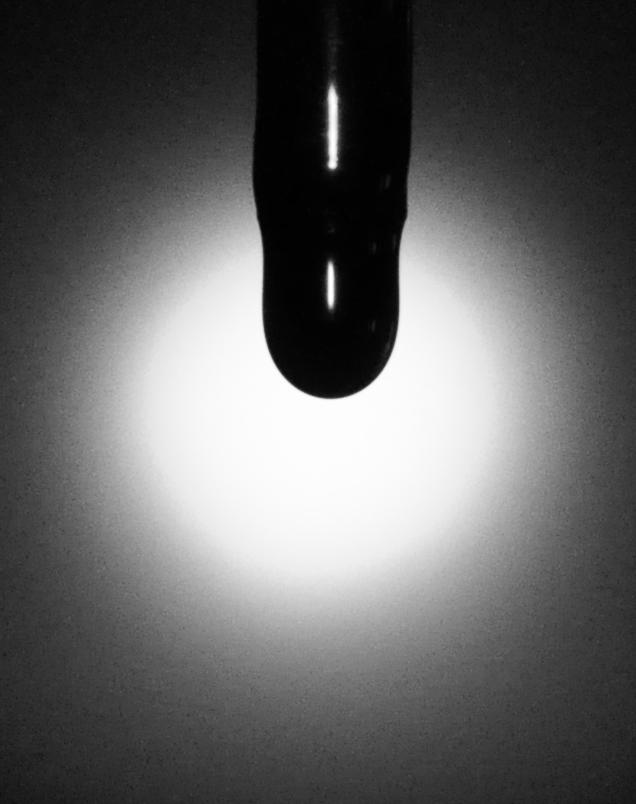
\includegraphics[height=84pt]{photogoutte4}} ;
    \node[label] (e) at (siliconoiloptim.south west) {\subfig{e}} ;
  \end{tikzpicture}

  \caption{(\subfig{a}) Experimental set-up for pendent drop surface
    tension measurement: a drop is hanging from a capillary tube
    (diameter here: $1.68\,$mm). A light source far behind the drop
    provides a bright background against which the drop is
    photographed. (\subfig{b,c}) Drops of water and perfluorated oil
    close to the maximum volume before drop detachment. It is easy to
    see that the difference in surface tension has a tremendous effect
    on the drop shape. The pendent drop method consists in exploiting
    this strong dependency in order to determine an unknown surface
    tension. (\subfig{d,e}) After improving experimental conditions to
    get rid of spurious reflections and to enhance contrast.}
  \label{fig:pendentdropphoto}
\end{figure}


\section{Introduction}
\label{sec:introduction}

The pendent drop method is commonly used to measure surface tensions
of liquids. It consists in analysing the shape of a drop hanging
typically from a capillary tube and about to detach. The method can
also be applied to drops resting on a flat surface. For transparent
liquids and in order to minimise interface contamination by adsorption
from the gas phase, one can also work with bubbles, again either
sessile or detaching from a tube. The shape of large drops or bubbles
results from a competition between gravity, which tends to lengthen
hanging drops or flatten sessile drops, and cohesive forces among
liquid molecules which tend to produce compact, spherical drops. As
shown in section~\ref{sec:theory}, the resulting drop profile
is described by only one non-dimensional parameter (tip radius over
capillary length), although in practice five parameters have to be
adjusted on a given image of a drop to account for unkown translation,
rotation, scale and drop volume. In the Plugin presented here for
example, the five parameters are the tip position and curvature, the
tilt of symmetry axis and the capillary length. The profile determined
this way gives access, besides to the surface tension, to other drop
properties such as volume or surface area.

While both the theory and the set-up are rather simple and
straightforward, to get precise, reliable and trustworthy results
requires some care in experimental details. Note for example that
surface tension depends quadratically on the capillary length, so that
any error in the length measurements will result in twice that
relative error on the surface tension:

\[
\gamma = \rho g \ell^2 \qquad \Rightarrow \qquad
\frac{\Delta\gamma}{\gamma} = 2 \frac{\Delta\ell}{\ell}
\]

The pendent drop technique is well established and there are numerous
high quality commercial devices to measure not only static, but also
dynamic properties of interfaces. These are however often available
only in laboratories specialised in interface physics and chemistry.
Here we show that within a few hours and with readily available and
cheap material, high quality measurements can be achieved. This is not
only useful to the biologist, geologist or environmental scientist who
stumbles onto a case where surface tension is a crucial parameter, but
also enables college or high school teachers to explore the
fascinating physico-chemistry of interfaces and surfactants (an
example of surfactant adsorption dynamics is presented below).

As a rough rule, if a \SIrange{2}{5}{\percent} uncertainty on the
surface tension is acceptable, a very simple set-up using a web-cam
and a light source a metre away should be sufficient. This article
describes a slightly more involved optical set-up using parallel light
and a macro objective, and underlines the pitfalls that must be
avoided in order to get a result that should be well within about
\SI{1}{\percent} of the true value. As always in metrology the
experimental difficulty increases very quickly with the desired
precision, as more and more small physical phenomena start having a
noticeable effect on the measurement. Relative uncertainties of and
below \num{1e-3} are beyond the scope of this article, requiring an
improved set-up with a telecentric objective and much better control
of the atmosphere, temperature, vapour pressure, vibrations \textit{et
  c{\ae}tera} than was attempted by the authors.

The structure of this article is as follows: the two following
sections~\ref{sec:bench} and \ref{sec:validation} describe the
measurement bench and present data measured with the Plugin in
comparison to reference data. Sections~\ref{sec:theory} and
\ref{sec:numerics} describe the underlying theoretical framework and
the plugin's inner architecture, respectively.
Appendix~\ref{sec:prerequisites} summarises the properties that the
input image must have for the Plugin to give meaningful results, and
the appendices~\ref{sec:usage} and \ref{sec:installation} contain
usage and installation instructions for the \gouttependante surface
tension measurement Plugin for ImageJ.


\section{Measurement bench}
\label{sec:bench}

Our measurement set-up is depicted in fig.~\ref{fig:setup}. The
condenser is at its focal length from the light source diaphragm, so
that light rays are parallel to the optical axis in the limit of a
closed diaphragm. The camera is focalised on the drop. The drop is
extruded either from a Pasteur pipette, or from a micropipette plastic
tip. The pipette is connected to a syringe that is driven either by
hand or by a syringe pump.

\begin{figure}
  \centering
  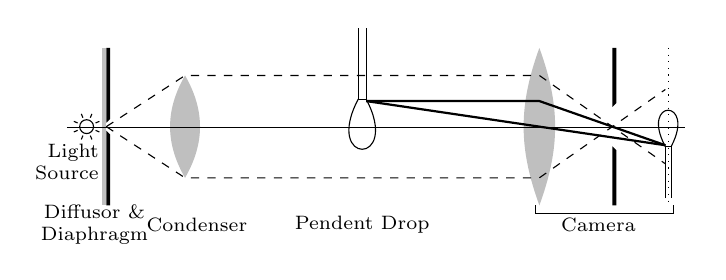
\begin{tikzpicture}[scale=0.5]
    \scriptsize % affects text nodes in this picture
    \draw (0,0) circle (5pt); % source de lumière
    \foreach \phi in { 22.5, 67.5, 112.5, 157.5 } { \draw (\phi:7pt)
      -- (\phi:10pt) ; \draw (-\phi:7pt) -- (-\phi:10pt) ; }
    \fill[gray!50] (0.4,-2) rectangle (0.5,2) ; % diffuseur
    % diaphragme source
    \fill (0.5,-2) -- ++(0.1,0) -- ++(0,1.8) -- +(-0.1,0.1) --
    cycle; \fill (0.5,2) -- ++(0.1,0) -- ++(0,-1.8) -- +(-0.1,-0.1)
    -- cycle; \fill[gray!50] (2.5,1.3) to [bend left] (2.5,-1.3) to
    [bend left] cycle; % lentille condenseur
    \draw (6.9,2.5)--(6.9,0.7)--(7.1,0.7)--(7.1,2.5); % tube
    \draw (6.9,0.7) .. controls (6,-1) and (8,-1) ..
    (7.1,0.7); % goutte
    \begin{scope}[yscale=-0.944/1.3] % tube et goutte image
      \draw (14.7,2.5)--(14.7,0.7)--(14.845,0.7)--(14.845,2.5);
      \draw (14.7,0.7) .. controls (14.04,-1) and (15.5,-1) ..
      (14.845,0.7);
    \end{scope}
    \draw[dotted] (14.77,2.0) -- +(0,-4.0); % capteur cmos
    % diaphragme camera
    \fill (13.455,2.0) -- ++(-0.1,0) -- ++(0,-1.5) -- ++(0.1,0.1) --
    cycle; \fill (13.455,-2.0) -- ++(-0.1,0) -- ++(0,1.5) --
    ++(0.1,-0.1) -- cycle;
    % lentille camera
    \fill[gray!50] (11.5,2.0) to [bend left=20] ++(0,-4) to [bend
    left=20] cycle;

    \draw[ultra thin] (-0.5,0)--(15.2,0); % axe optique
    % rayons
    \draw[dashed] (0.5,0)--(2.5,1.3)--(11.5,1.3)--(14.7,-0.944);
    \draw[dashed] (0.5,0)--(2.5,-1.3)--(11.5,-1.3)--(14.7,0.944);
    \draw[thick] (7.1,0.65)--(14.7,-0.472); % rayon objet
    \draw[thick] (7.1,0.65)--(11.5,0.65)--(14.7,-0.472);

    % legendes
    \node[align=right] at (-0.5,-0.9) {Light\\Source};
    \node[align=center] at (0.2,-2.5) {Diffusor \&\\Diaphragm};
    \node at (2.8,-2.5) {Condenser} ; \node at (7,-2.5) {Pendent
      Drop}; \draw[ultra thin] (11.4,-2.0) -- ++(0,-0.2) --
    ++(3.5,0) -- ++(0,0.2) ; \node at (13,-2.5) {Camera};
  \end{tikzpicture}
  
  \caption{Schematics of a simple surface tension measurement set-up.
    The horizontal distances are much larger than depicted, both the
    light source and the camera being at about \SI{30}{\centi\metre}
    from the drop, while the condenser lens has a diameter of
    \SI{25}{\milli\metre}. We use a commercial DSLR camera with a
    Zeiss \SI{50}{\milli\metre} Macroplanar objective, and a light
    emitting diode as a light source.}
  \label{fig:setup}
\end{figure}

This basic measurement bench is quite easy to set up. It can even be
simplified further by replacing the light source and condenser by a
bright screen at a large distance from the drop. In any case the drop
appears dark against a light background, because even for transparent
liquids light rays traversing the drop will be refracted at the
interface and miss the camera entrance pupil (except at the very
center of the drop, where a small image of the light source can be
seen because the interfaces are perpendicular to the optical axis). 

\begin{figure}
  \centering
  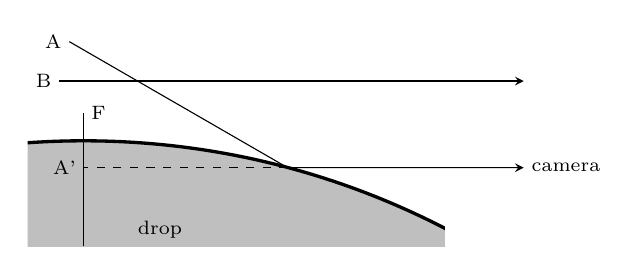
\begin{tikzpicture}
    \scriptsize % affects text nodes in this picture
    \newcommand{\dphi}{15}
    \newcommand{\rad}{10}
    \coordinate (dropcenter) at (-90-\dphi:\rad) ;
    % light rays
    \draw[->,>=stealth] (180-2*\dphi:3.2) node[left] {A} -- (0,0) -- (3,0) node[right] {camera} ;
    \draw[->,>=stealth] (-2.9,1.1) node[left] {B} -- (3,1.1) ;
    % drop
    \clip (-3.3,1) rectangle (2,-1) ;
    \fill[gray!50,draw=black,very thick] (dropcenter) circle [radius=\rad] ;
    \node[above right] at (-2,-1) {drop} ;
    % virtual light ray
    \draw[dashed] (0,0) -- (0,0 -| dropcenter) node[left] {A'} ;
    % focal plane
    \draw[very thin] (dropcenter |- 0,-1) -- +(0,1.7) node[right] {F} ;
  \end{tikzpicture}
  \caption{Light reaching the drop from direction A will be partially
    reflected towards the camera, whose focal plane cuts through the
    drop at $F$. The light will appear as coming from point $A'$, and
    be almost as bright as direct light from e.g. $B$, because the
    reflection coefficient tends to unity for near grazing incidence.
    As a result, the drop may appear slimmer than it is.}
  \label{fig:grazing}
\end{figure}

Despite the simplicity of the set-up is important however to be aware
of a few effects that can affect the measurement quality. The drop can
indeed appear smaller than its real size for several reasons. One
consists in grazing reflections at the border of the drop
(fig.~\ref{fig:grazing}). For incident angles above about \ang{82} on
water for example, the reflected intensity lies above
\SI{50}{\percent} of the incident intensity, so that the corresponding
points on the drop will be classified as outside. This corresponds to
an error on the drop radius of about \SI{1}{\percent}, and therefore
an error on the surface tension of \SI{2}{\percent}. Note that the
error on the surface tension is most likely even larger, because
eroding the drop image by a few pixels does not amount to a mere
change in scale: the drop's vertical extent is usually larger than its
horizontal diameter, so that eroding sides and bottom by the same
amount of pixels will change its aspect ratio and lead to an
unphysical profile that cannot even be accurately adjusted by the
Young-Laplace equation any more.

The condenser set-up prevents this source of errors by providing only
near-parallel light rays. Alternatively this selection of light
parallel to the optical axis can also be achieved by a telecentric
lens on the camera side, as this type of lens is precisely built to
have its aperture stop virtually infinitely far from the imaged
object. Using a telecentric lens comes with the added benefit of
having a magnification which is independent of the drop's distance to
the camera, thereby reducing potential errors when calibrating the
image scale. The commercial apparatus against which we validate our
measurement bench and numerical analysis (see next section) uses such
a telecentric lens, and a simple back-lit ground glass as an extended
omnidirectional light source.

Errors also arise from oversaturating the image sensor, for two
reasons. One is that common CCD and CMOS sensors present some degree
of blooming, meaning that electrons from oversaturated pixel wells
overflow into adjacent pixels and/or fail to completely transfer
(mainly in the case of CCDs) during pixel read-out, causing
neighbouring pixels (\textit{viz} pixels in the same column) to appear
much brighter than they should. The second reason is that our Plugin
puts the drop interface at half the intensity contrast between drop
and background. If the background intensity is oversaturated and the
captured picture therefore presents intensities clipped to values
below a maximum, the \SI{50}{\percent} threshold on the (clipped)
pixel values amounts to a lower threshold on the real intensity
interval, again effectively shifting the drop contour inwards. To
prevent these effects the background illumination must be as uniform
as possible, and the camera aperture and exposure time chosen so as
not to saturate the sensor.


\section{Validation measurements}
\label{sec:validation}

The following table compares capillary length measurements for three
liquids (water, hexadecane and mercury) using our set-up and sofware
with values from the literature and values measured using a commercial
apparatus (Teclis Instruments: Tracker, software version 9.7.0).
Additionally, we report the capillary length that our software
determines from images taken on the commercial apparatus. In all cases
the indicated uncertainty is the standard deviation of three to twelve
drops, each measured two to four times (varying lighthing, exposure
settings and the part of the drop to which the theoretical contour was
adjusted). Mercury vapour represents a health hazard, and its vapour
pressure depends strongly on the temperature\cite{mercury}.
Considering the high summer temperatures of around \SI{30}{\celsius},
we refrained from performing measurement of mercury drops using the
commercial apparatus which could not easily be relocated. We could
however transfer our bench to an air-conditioned room to perform the
measurement on mercury at about half the vapour pressure.

\begin{table}
  \begin{tabular}{c|c c c}
    & water & hexadecane & mercury \\
    Temperature & \SI{303}{K} & \SI{303}{K} & \SI{295}{K} \\
    Density & \SI{995.7}{kg/m^3}\cite{danslax} & \SI{767.7}{kg/m^3}\cite{rho_hexadecane} & \SI{13541}{kg/m^3}\cite{danslax} \\
    \hline
    capillary length \dots \\
    from literature &
    \SI{2.70}{mm}\cite{danslax}
    & \SI{1.885}{mm}\cite{gamma_hexadecane} &
    \SI{1.89}{mm} (\SI{293}{\kelvin})\cite{danslax}
    \\\\
    imaging and analysis: & \SI{2.703}{mm} & \SI{1.863}{mm} & \SI{1.70}{mm} \\
    our set-up and sofware & $ \pm \SI{0.015}{mm} $ & $ \pm \SI{0.018}{mm} $ & $ \pm \SI{0.015}{mm} $ \\\\
    imaging and analysis: & \SI{2.697}{mm} & \SI{1.882}{mm} & --- \\
    commercial apparatus & $ \pm \SI{0.01}{mm} $ & $\pm \SI{0.02}{mm} $ \\\\
    imaging: com. apparatus & \SI{2.750}{mm} & \SI{1.890}{mm} & --- \\
    analysis: our software & $\pm \SI{0.01}{mm} $ & $\pm \SI{0.03}{mm} $ \\\\
  \end{tabular}
  \caption{Comparison of capillary lengths of three liquids from different sources.}
\end{table}

Our measurements for water and hexadecane agree with literature values
as well with the values obtained through the commercial apparatus. The
measurements for mercury yield a capillary length about
\SI{10}{\percent} lower than expected. We suspect that oxidation of
its surface in air may have been responsible for lowering the surface
tension. Analysing the images from the commercial apparatus with our
software slightly overestimates the capillary length of water,
possibly to a small error on the independently performed image scale
calibration. In any case, all measurements for water and hexadecane
differ by less than \SI{1}{\percent}, giving a conservative estimate
of the precision of our set-up and analysis.

\subsection{Example of slow surfactant dynamics}

If the surface tension varies over time, the measurement of the
surface tension on successive images can be performed efficiently by
taking each result of a fit as a starting guess for the adjustment of
the following image, which is what the \gouttependante Plugin will do
automatically if run on a stack. Fig.~\ref{fig:surfactine} shows the
time evolution of the capillary length and surface tension of an
acqueous solution of surfactine, a lipopeptidic bio-surfactant
(molecular weight \SI{1e3}{\dalton}) produced by the bacteria
\textit{B.~subtilis}. When the drop is initially extruded from the
capillary, fresh interface is created that is only weakly populated
with surfactant molecules, so that the surface tension is close to
that of pure water. Over time surfactant molecules diffusing in the
liquid reach the free surface and adsorb to the interface. It takes
several minutes for the molecule concentration at the interface to
reach an equilibrium.

\begin{figure}
  \centering
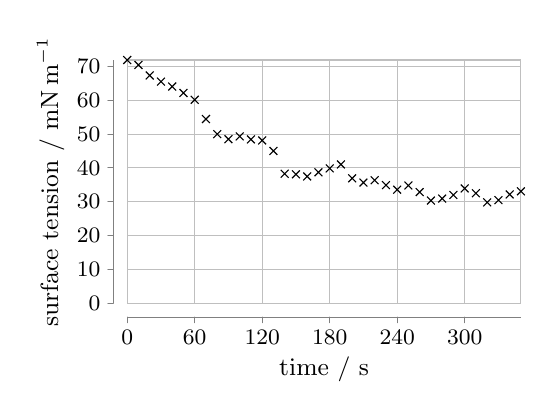
\begin{tikzpicture}
  \datavisualization [ scientific axes=clean ,
x axis={attribute=time, grid, ticks={step=60}, label={time / \si{\second}}},
y axis={attribute=surface tension, include value=0, grid,
  label={surface tension / \si{\milli\newton\per\metre}}},
style sheet=strong colors,
visualize as scatter ]
%data [read from file=Surfactine_954_2015-07-13-3.csv] ;
data {
time, capillary length, surface tension
0, 2.71, 71.87
10, 2.68, 70.41
20, 2.62, 67.3
30, 2.58, 65.5
40, 2.55, 64.04
50, 2.52, 62.13
60, 2.48, 60.13
70, 2.36, 54.44
80, 2.26, 49.97
90, 2.22, 48.48
100, 2.24, 49.31
110, 2.22, 48.41
120, 2.21, 48.11
130, 2.14, 45.01
140, 1.98, 38.27
150, 1.97, 38.11
160, 1.95, 37.47
170, 1.99, 38.7
180, 2.02, 39.86
190, 2.04, 41.02
200, 1.96, 36.92
210, 1.91, 35.67
220, 1.93, 36.36
230, 1.89, 34.92
240, 1.85, 33.56
250, 1.88, 34.81
260, 1.83, 32.86
270, 1.76, 30.36
280, 1.78, 30.94
290, 1.81, 32.0
300, 1.86, 33.93
310, 1.82, 32.52
320, 1.74, 29.82
330, 1.76, 30.48
340, 1.81, 32.16
350, 1.84, 33.08
};
\end{tikzpicture}

\caption{Surface tension of a drop of surfactine solution over time.}
\label{fig:surfactine}
\end{figure}

The irregular decrease of the surface tension, especially the sudden
drops around $t=\SI{70}{\second}$ and $t=\SI{130}{\second}$ are not
due to measurement errors, but to variations of the drop volume by the
human operator. Recall that for a reliable surface tension measurement
the curvature must vary significantly from top to bottom, therefore
the drop size needs to be of the order of the capillary length.
However the drop is then also close to pinch-off because the maximum
drop size before pinch-off is of the order of $(d\ell_c^2)^{1/3}$
where $d$ is the tube diameter. As the surface tension, and thus
$\ell_c$, decreases over time in the case of the surfactine drop, the
drop volume has to be diminished to prevent pinch-off, by pulling
liquid back into the capillary tube before the drop becomes unstable.
This reduces the free surface and increases the surface density of
surfactant molecules, which in turn results in a further decrease of
the surface tension. On the other hand, if the drop volume is
increased as around $t=\SI{180}{\second}$, the drop surface also
increases and the surfactant is diluted at the interface, increasing
the surface tension. In order to measure the change in surface tension
excusively due to adsorption of new surfactant molecules, a feedback
loop is needed that maintains a constant drop surface.


\section{Physics of the pendent drop}
\label{sec:theory}

Cohesive forces between the molecules of the liquid prevent the
pendent drop from detaching under its weight, up to a critical size.
The effect of these cohesive forces is thermodynamically described by
a contribution $\gamma\, \ud S$ to the free energy that is
proportional to the surface variation $\ud S$, where $\gamma$ is the
surface free energy or surface tension. In other words, cohesion is
accounted for by considering that the free surface of a liquid is
under tension, and the equilibrium shape is one minimising this
surface together with the potential energy.

To establish an equation describing the shape of an axisymmetric
pendent drop (fig.~\ref{fig:notations}), it is easier to consider the
local pressure balance. Just like the pressure inside of a rubber
balloon is higher than outside, surface tension is responsible for a
pressure jump across a curved interface, that is related to its mean
curvature $\bar\kappa$ by Young-Laplace's formula $\Delta\! p(z) =
\gamma \bar\kappa(z)$.

Now in a pendent drop the pressure jump across the interface varies
with height, because of the density difference between the inner
liquid and outer gas phase, implying that the surface curvature must
vary as well. Indeed, the drop has an equilibrium shape if and only if
the hydrostatic pressure difference is everywhere equal to the
Young-Laplace pressure jump across the interface.

Take the lowest point of the drop as origin for the height coordinate
$z$. Then the pressure inside the drop is $p_{\mathrm{in}}(z=0) -
\rho_{\mathrm{in}} g z$ at a distance $z$ above it, while it is
$p_{\mathrm{out}}(z=0) - \rho_{\mathrm{out}} g z$ outside at the same
height. $g$ denotes gravitational acceleration and
$\rho_{\mathrm{in/out}}$ the densities of the respective phases.
Noting $\Delta\! p_0 = p_{\mathrm{in}}(z=0) - p_{\mathrm{out}}(z=0)$
the pressure drop at the drop tip, and $\Delta\!\rho =
\rho_{\mathrm{in}} - \rho_{\mathrm{out}}$ the density contrast, we
have a pressure jump across the interface $\Delta\! p(z) = \Delta\!
p_0 - \Delta\!\rho g z$ at height $z$. Note that the value of
$\Delta\! p_0$ is unkown beforehand. It depends on the geometry of our
set-up and the drop volume, and constitutes an integration constant.

\begin{figure}
  \begin{captionbeside}{Notations. The drop profile is assumed to be
      axisymmetric, and is described by the two cylindrical coordinates
      $R(s)$ and $Z(s)$ as a function of the curvilinear parameter
      $s$. The local tilt $\psi$ with respect to the axis normal
      enters the expression for the interface curvature, and is
      related to $R$ through $R' = \cos\psi$. We have spherical
      symmetry at the very tip, with radius $r_0$.}
\begin{tikzpicture}
  %\grid{3cm}{3cm}
  \pgftext{\pgfimage[height=15em]{dropsketch}}
  \pgftext[bottom,right,x=-10mm,y=-6mm] {$r_0$}
  \pgftext[right,x=-5mm,y=-13mm] {$Z$}
  \pgftext[bottom,x=3mm,y=-9mm] {$R$}
  \pgftext[bottom,left,x=18mm,y=-7mm] {$\psi$}
  \pgftext[x=-9mm,y=11mm] {$\rho_{\mathrm{in}}$}
  \pgftext[x=-20mm,y=11mm] {$\rho_{\mathrm{out}}$}
\end{tikzpicture}
\end{captionbeside}
\label{fig:notations}
\end{figure}

At equilibrium, this hydrostatic pressure jump is equal to the Laplace
pressure given above: $\Delta\! p_0 - \Delta\!\rho g z = \gamma
\bar\kappa(z)$. We parametrise the drop surface in cylindrical
coordinates as $(R(s), Z(s))$, where $s$ is the curvilinear distance
to the tip along the interface. Expressing the mean curvature as a
function of $R$, $Z$ and the angle $\psi$ between the tangent plane to
the interface and the horizontal: $\ud R/\ud s = \cos\psi$, one obtains
the following expression for the pressure equilibrium:

\[\label{eq:shape}
  - \frac{1}{\ell_c^2} \sin\psi =
  \frac{\ud}{\ud s}\left( \frac{\ud\psi}{\ud s} + \frac{\sin\psi}{R} \right).
\]

 The boundary conditions at the drop tip are $\psi(0)=0$ and $\ud\psi
/ \ud s = p(0)/2\gamma = 1/r_0 = \mathrm{const.}$, where $r_0$ is the
radius of curvature of the drop tip which has locally spherical
symmetry. Scaling all lengths by the characteristic length $\ell_c =
\sqrt{\gamma/\Delta\!\rho g}$ (called \emph{capillary length}) yields
one universal drop shape equation

\begin{equation}\label{eq:shapeNonDim}
  - \sin\psi =
  \frac{\ud}{\ud s}\left( \frac{\ud\psi}{\ud s} + \frac{\sin\psi}{R} \right)\\
  \mbox{with } \psi(0)=0 \mbox{ and } \psi'(0) = \ell_c/r_0,
\end{equation}

Note that the solutions (i.e. all possible axisymmetric drop shapes)
are fully determined by the choice of the initial condition for
$\psi'(0)$, which is just the ratio of the capillary length and the
radius of curvature of the drop tip.

\section{What the Plugin does internally}
\label{sec:numerics}

\minisec{numérical integration}
The equation~(\ref{eq:shapeNonDim}) is integrated for a given parameter
$\ell_c/r_0 = 1/r_*$ using a fourth order Runge-Kutta scheme. Near the
drop tip the integral equation becomes singular as $R\to 0$, but the
solution itself is perfectly regular: it is simply a nearly perfectly
spherical profile (at least at distances small with respect to
capillary length and tip radius). We can thus use an analytical
solution to get away from the singularity at $R=0$. The leading order
terms of that solution are

\[
\left.%
\begin{array}{lll}
R & = & r_*\sin\frac{s}{r_*} + \frac{s^5}{40 r_*^2} + O(s^6) \\
Z & = & \frac{1}{2r_*} s^2 (1 + (\frac{1}{16} - \frac{1}{12r_*^2}) s^2) + O(s^6)\\
\psi & = & s/r_* (1-s^2/8) + O(s^5)
\end{array}\right\}
\mathrm{for}\quad s \ll 1 \wedge s \ll r_*
\]

We use this solution to calculate the first piece of drop contour
where $s \ll 1$ and $s \ll r_*$. Then we continue through numerical
integration.

\minisec{matching the theoretical solution to the image of the drop}
The drop contour from the previous integration is then rescaled,
translated and rotated according to the given parameters (tip
position, curvature, and gravity angle) to be compared to the
experimental drop image. A distance between this theoretical contour
$\mathcal{C}$ and the observed drop border $\mathcal{B}$, is then
calculated as the sum, over all pixel rows and both sides of the drop,
of the difference of horizontal positions:

\[
\chi^2 = \sum_{z} |x_{\mathcal{C},\mathrm{left}}(z) - x_{\mathcal{B},\mathrm{left}}(z)|^2 +
|x_{\mathcal{C},\mathrm{right}}(z) - x_{\mathcal{B},\mathrm{right}}(z)|^2
\]

The drop border $\mathcal{B}$ is detected beforehand by matching a
step-function to the image intensity profile in a neighbourhood of the
interface.

\minisec{optimize by varying parameters and iterating} In case
automated fitting of some parameters is requested (by pressing the
``fit'' or the ``OK'' button), the Plugin tries to minimise the
distance function $\chi^2$ using an algorithm by
Powell~\cite{Powell1965,Brandt1992}. This algorithm consists in
successively varying each parameter, searching for each the value that
will yield the best-fitting integrated drop contour. The user can
choose which parameters are adjusted in this prodecure, and which ones
are kept fixed. After all free parameters have been varied, the
algorithm checks whether it is not more efficient to minimise along
another direction in parameter space, i.e. modify several parameters
concurrently, and possibly updates the list of directions. The whole
process is repeated until the change in the fit distance $\chi^2$
after a full round becomes too small.


\appendix


\section{Prerequisites}
\label{sec:prerequisites}

The Plugin is run on a high contrast image of a pendent drop
(Fig.~\ref{fig:usage}-left). Pixel values are expected to be close to
zero within the drop, and close to saturation (i.e. 255 for 8-bit
images) outside. This is typically obtained by taking the picture of
the drop in front of a light background far away from the drop
(Fig.~\ref{fig:pendentdropphoto}). Bright spots well within the drop
are not a problem, but contrast should be good in the vicinity of the
contour. Note however that saturation should be avoided at all cost,
both because of blooming effects in the light sensitive image
recording device and because it tends to bias the interface detection
towards the inside of the drop. See also section~\ref{sec:bench}.


\section{Pendent\_Drop ImageJ Plugin Usage}
\label{sec:usage}

By default, the \gouttependante Plugin appears in the Plugins menu of
ImageJ, in a folder termed \texttt{Drop Analysis}. The menu item
\texttt{About Pendent Drop} will show a bit of information on the
Plugin, including usage, the update site and an example image on which
you can test the Plugin. The menu item \texttt{Pendent Drop} launches
the Plugin itself.

\begin{figure}
  \centering
  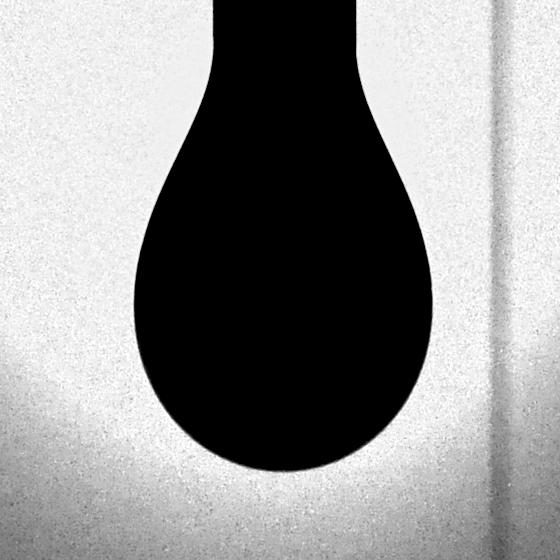
\includegraphics[width=0.28\textwidth]{eauContrasteMax}\hfill
  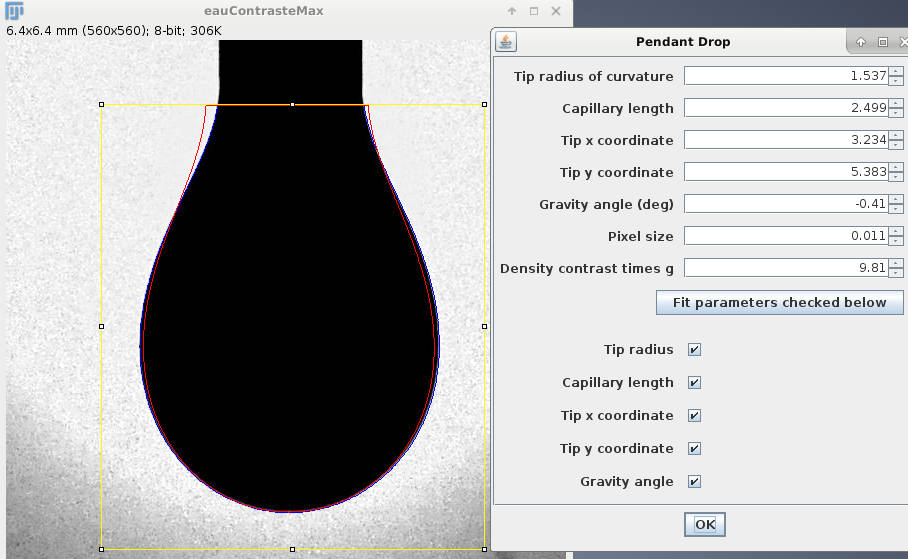
\includegraphics[width=0.455\textwidth]{eauContrasteMaxInitial}\hfill
  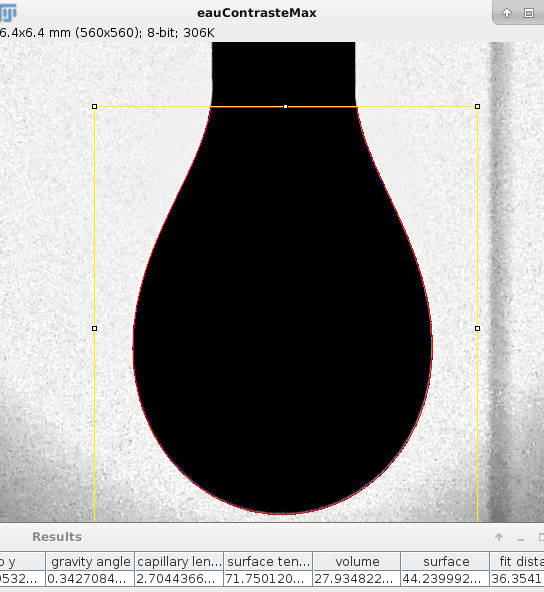
\includegraphics[width=0.258\textwidth]{eauContrasteMaxFit}
  \caption{Plugin usage. \textbf{(left)} starting image, contrasted
    just short of saturating black and white levels. \textbf{(middle)}
    image with rectangular ROI selection and initial guess next to
    Plugin dialog. \textbf{(right)} The profile after automatic
    optimisation of the parameters.}
  \label{fig:usage}
\end{figure}

Draw a rectangular Region Of Interest (ROI) around the pendent drop
before calling the Plugin (Fig.~\ref{fig:usage}-middle). The ROI
should not include the inlet tube, but only the free surface of the
drop. A few ten or so pixels margin around the drop is sufficient for
the interface detection to perform correctly.

Fill in any parameter values you know, and check the plausibility of
the initial guess for the others. If the image was calibrated for
spatial scale, the corresponding scale is proposed by the Plugin and
all length scales are expressed in calibrated units. If the image is
not calibrated all lengths are given in pixels, including the
resulting capillary length. The angle specifies the tilt of the
symmetry axis away from the vertical, in degrees. 

Two overlays are shown on the image: a blue line indicating the drop
border as detected by the Plugin, and a red line representing the
profile described by the current parameter values.

a) modify the parameters so as to improve the visual accordance of
theoretical profile and image. In version 2.0.0 of the Plugin a
measure of the distance between profile and border is logged to the
console, it should be made as small as possible.

b) check those parameters that the Plugin may adjust and click on the
button for automatic minimisation. Only the previously checked
parameters are varied when trying to find an optimal shape. The
overlay is updated accordingly. Note that the minimisation algorithm
can get trapped in a local minimum, so try starting from different
initial values and compare the results. Also check whether the
resulting profile looks satisfactory.

Clicking the \texttt{OK} button will cause the Plugin to fit each
slice of the active stack by a drop profile. The dialog parameters
serve as starting point for the fit of the first slice, while
subsequent slices are adjusted starting from the result of the
previous slice. The resulting drop shape descriptors, surface tension
and drop properties (volume, surface) for each slice are summarised in
a result table.

\paragraph{How to get the surface tension}
If the image was scale-calibrated, and a sensible value was entered
for the `\texttt{density contrast times g}' parameter (the difference
of the densities in/outside the drop multiplied by your planet's
gravitational acceleration, $(\rho_{\mathrm{in}}-\rho_{\mathrm{out}})g
= \Delta\rho\,g$), then the surface tension is indicated in physical
units. For example if the \texttt{pixel size} is in millimetres per
pixel, and the \texttt{density contrast times g} is in grams per
square second and square millimetre (e.g.\ around
\SI{9.8}{\gram\per\square\milli\metre\per\square\second} for water in
air on earth), then the indicated surface tension is in
\si{\gram\per\square\second} or milli-Newton per metre. Otherwise the
unit conversion has to be performed by hand. Recall that surface
tension $\gamma$ is calculated from the capillary length using the
formula $\gamma = \Delta\!\rho g \ell_c^2$.


\section{Installing the Pendent\_Drop Plugin for ImageJ}
\label{sec:installation}

\begin{description}
\item[via the update site] The preferred method is to use
  \href{http://fiji.sc/}{Fiji}'s \cite{FijiSite,Schindelin2012} update
  mechanism. Detailed step-by-step instructions with illustrations can
  be found at
  \url{http://fiji.sc/How_to_follow_a_3rd_party_update_site}. This
  software is hosted at \url{http://fiji.sc/List_of_update_sites}.

  In the \texttt{Help} menu, select \texttt{Update Fiji} to start the
  updater. Choose the \texttt{Advanced mode}, click on \texttt{Manage
    update sites} and add a site with the following URL:
  \begin{center}
    \url{http://sites.imagej.net/Daerr/}
  \end{center}
  (The name has no particular importance, choose something meaningful
  to you)

  Enable this site (check the box next to it) and close the window to
  get back to the main updater window. In the list of Plugins, locate
  \texttt{plugins:pendent\_drop-2.0.0.jar} (to find it more easily you
  can restrict the list to items from the new site using the menu
  above the list), select it and mark it for installation. Apply
  changes, restart Fiji: a new folder \texttt{Drop Analysis} should
  appear in the Plugins menu.

\item[by downloading the jar file] For a manual installation, and as
  usual with ImageJ Plugins, just put the jar into ImageJ's
  \texttt{plugins} folder or a subfolder thereof. Restart ImageJ to
  see the Plugin.

\item[by building from the source] The source code of the
  \gouttependante Plugin is hosted on gitlab at
  \url{https://github.com/adaerr/pendent-drop}. You will need
  tools such as \texttt{git} and a java compiler and be familiar with
  their usage. If you are using \texttt{maven}, then the command
  \texttt{mvn package} should produce a jar file for you in the
  \texttt{target} directory. Check the git history to identify usable
  states that you can check out and compile.

\end{description}


\begin{thebibliography}{9}

\bibitem{ImageJ} W. S. Rasband, \textit{ImageJ}, U. S. National
  Institutes of Health, Bethesda, Maryland, USA,
  \url{http://imagej.nih.gov/ij/}, 1997-2010.
  
\bibitem{FijiSite} Fiji web site: \url{http://fiji.sc/}

\bibitem{Schindelin2012} J. Schindelin \textit{et al.}, \textit{Fiji: an
    open-source platform for biological-image analysis}, Nature
  Methods 9(7), pp.676--682 (2012)

\bibitem{Powell1965} M. J. D. Powell, \textit{Computer Journal}
  \textbf{7} (1965) 155

\bibitem{Brandt1992} S. Brandt, \textit{Datenanalyse}, BI-Wiss.-Verlag
  (Mannheim, Leipzig, Wien, Zürich) 3rd edition, ISBN 3-411-03200-6
  (1992)

\bibitem{mercury} F. M. Ernsberger and H. W. Pitman, \textit{New
    absolute manometer for vapor pressures}, Rev. Sci. Instrum.
  \textbf{26}(6): 584--589; 1955. M. L. Huber, A. Laesecke and D. G.
  Friend, \textit{The vapor pressure of Mercury}, NISTIR report 6643
  (2006), URL:
  \url{http://www.boulder.nist.gov/div838/SelectedPubs/NISTIR.6643.pdf}

% pages Hg 1-134f, 1-901 
% density: rho=13.541 g/cm³ @ 22 degC
% surface tension 476 mN/m @ 20 degC => l = 1.89 mm (rho=13.546 g/cm³ @ 20 degC)
%
% pages water: 1-600, 1-607
% density: rho=0.9957 g/cm³ @ 30 degC
% surface tension: 71.15 mN/m @ 30 degC => l = 2.699 mm
% 
% hexadecane: surface tension can only be estimated from the 
% Parachores tabulated p 1-1247f: P = 672.1
% with M = 114.2 g/mol, rho = 0.773 g/cm³ -> gamma = 27.7 mN/m, l = 1.91 mm
\bibitem{danslax} D'Ans and Lax, \textit{Taschenbuch für Chemiker und
    Physiker}, Springer, 1967 (3rd edition), pp.~1-134f, 1-600ff,
  1-607, 1-901

\bibitem{rho_hexadecane} S. S. Joshi, \textit{Thermodynamic Interactions in Mixtures of Bromoform with Hydrocarbons}, J. Phys. Chem. \textbf{95} (1991) 5299--5308

%\bibitem{gamma_eau&Hg1} web site : \url{https://fr.wikipedia.org/wiki/Tension_superficielle}
%
%\bibitem{gamma_eau&Hg2} web site : \url{http://tensionsuperficielle.free.fr/tension-superficielle/}
%
%\bibitem{gamma_eau} web site : \url{http://bernard.pironin.pagesperso-orange.fr/aquatech/mat-mol.htm}
%
%\bibitem{gamma_mercury} web site : \url{https://books.google.fr/books?id=Mhg0SNJoM5gC&pg=PA5&lpg=PA5&dq=longueur+capillaire+mercure&source=bl&ots=mhTmSt060B&sig=hRzV67Ve7vVXHMAdR-efKzsKPXY&hl=fr&sa=X&ved=0CD0Q6AEwBGoVChMImKG_6ubfxgIVh2sUCh1N0QDH#v=onepage&q=longueur%20capillaire%20mercure&f=false}

%  Taking the mean of the measurements in this article (one original
%  and three cited): gamma = 26.67 mN/m @ 303.15K
%  => l = 1.885 mm (with rho = 0.7767 g/cm^3)
\bibitem{gamma_hexadecane} L. I. Rolo, A. I. Caço, A. J. Queimada, I. M. Marrucho, and J. A. P. Coutinho, \textit{Surface tension of Heptane, Decane, Hexadecane, Eicosane and Some of Their Bianary Mixtures} J. Chem. Eng. Data \textbf{47} (2002), 1442--1445

%\bibitem{rho_eau1} web site : \url{http://www.atomer.fr/1/1-densite-eau.html}
%
%\bibitem{rho_eau2} web site : \url{http://www.thermexcel.com/french/tables/eau_atm.htm}
%
%\bibitem{rho_eau3} web site : \url{http://www.econologie.com/masse-volumique-de-l-eau-et-temperature-articles-4032.html}
%
%\bibitem{rho_mercury1} web site : \url{https://fr.wikipedia.org/wiki/Mercure_%28chimie%29}
%
%\bibitem{rho_mercury2} web site : \url{http://www.engineeringtoolbox.com/mercury-d_1002.html}
%
%\bibitem{rho_mercury3} web site : \url{https://en.wikipedia.org/wiki/Mercury_%28element%29}
%
%\bibitem{rho_hexadecane1} web site : \url{https://en.wikipedia.org/wiki/Hexadecane}
%
%\bibitem{rho_hexadecane2} web site : \url{http://www.ddbst.com/en/EED/PCP/DEN_C516.php}
%
%\bibitem{rho_hexadecane3} PubChem database, maintained by: NCBI,
%  National Institutes of Health,
%  \url{http://pubchem.ncbi.nlm.nih.gov/compound/hexadecane}


\end{thebibliography}

\end{document} 

%%% Local Variables: 
%%% mode: latex
%%% TeX-PDF-mode: t 
%%% End: 
